\chapter{Phase III}

\section{Structur of software}
The figure \ref{fig:phase3} shows the implementation details behind the \emph{Opponent Model Strategy}. The \emph{Opponent Logger} tracks all the actions that are made by all players and associates them with the context at which these actions have been made. These actions are stored as list of \emph{Opponent Entry}-objects. 

At the showdown all the players that are still in the game have to show their cards. Now the \emph{Opponent Entry}-list of these players is went through. The player's cards are combined with the share cards and the hand strength is computed. The hand strength is committed to the \emph{Opponent Model} together with the current context and the player's action.

\begin{figure}[h]
  \centering
  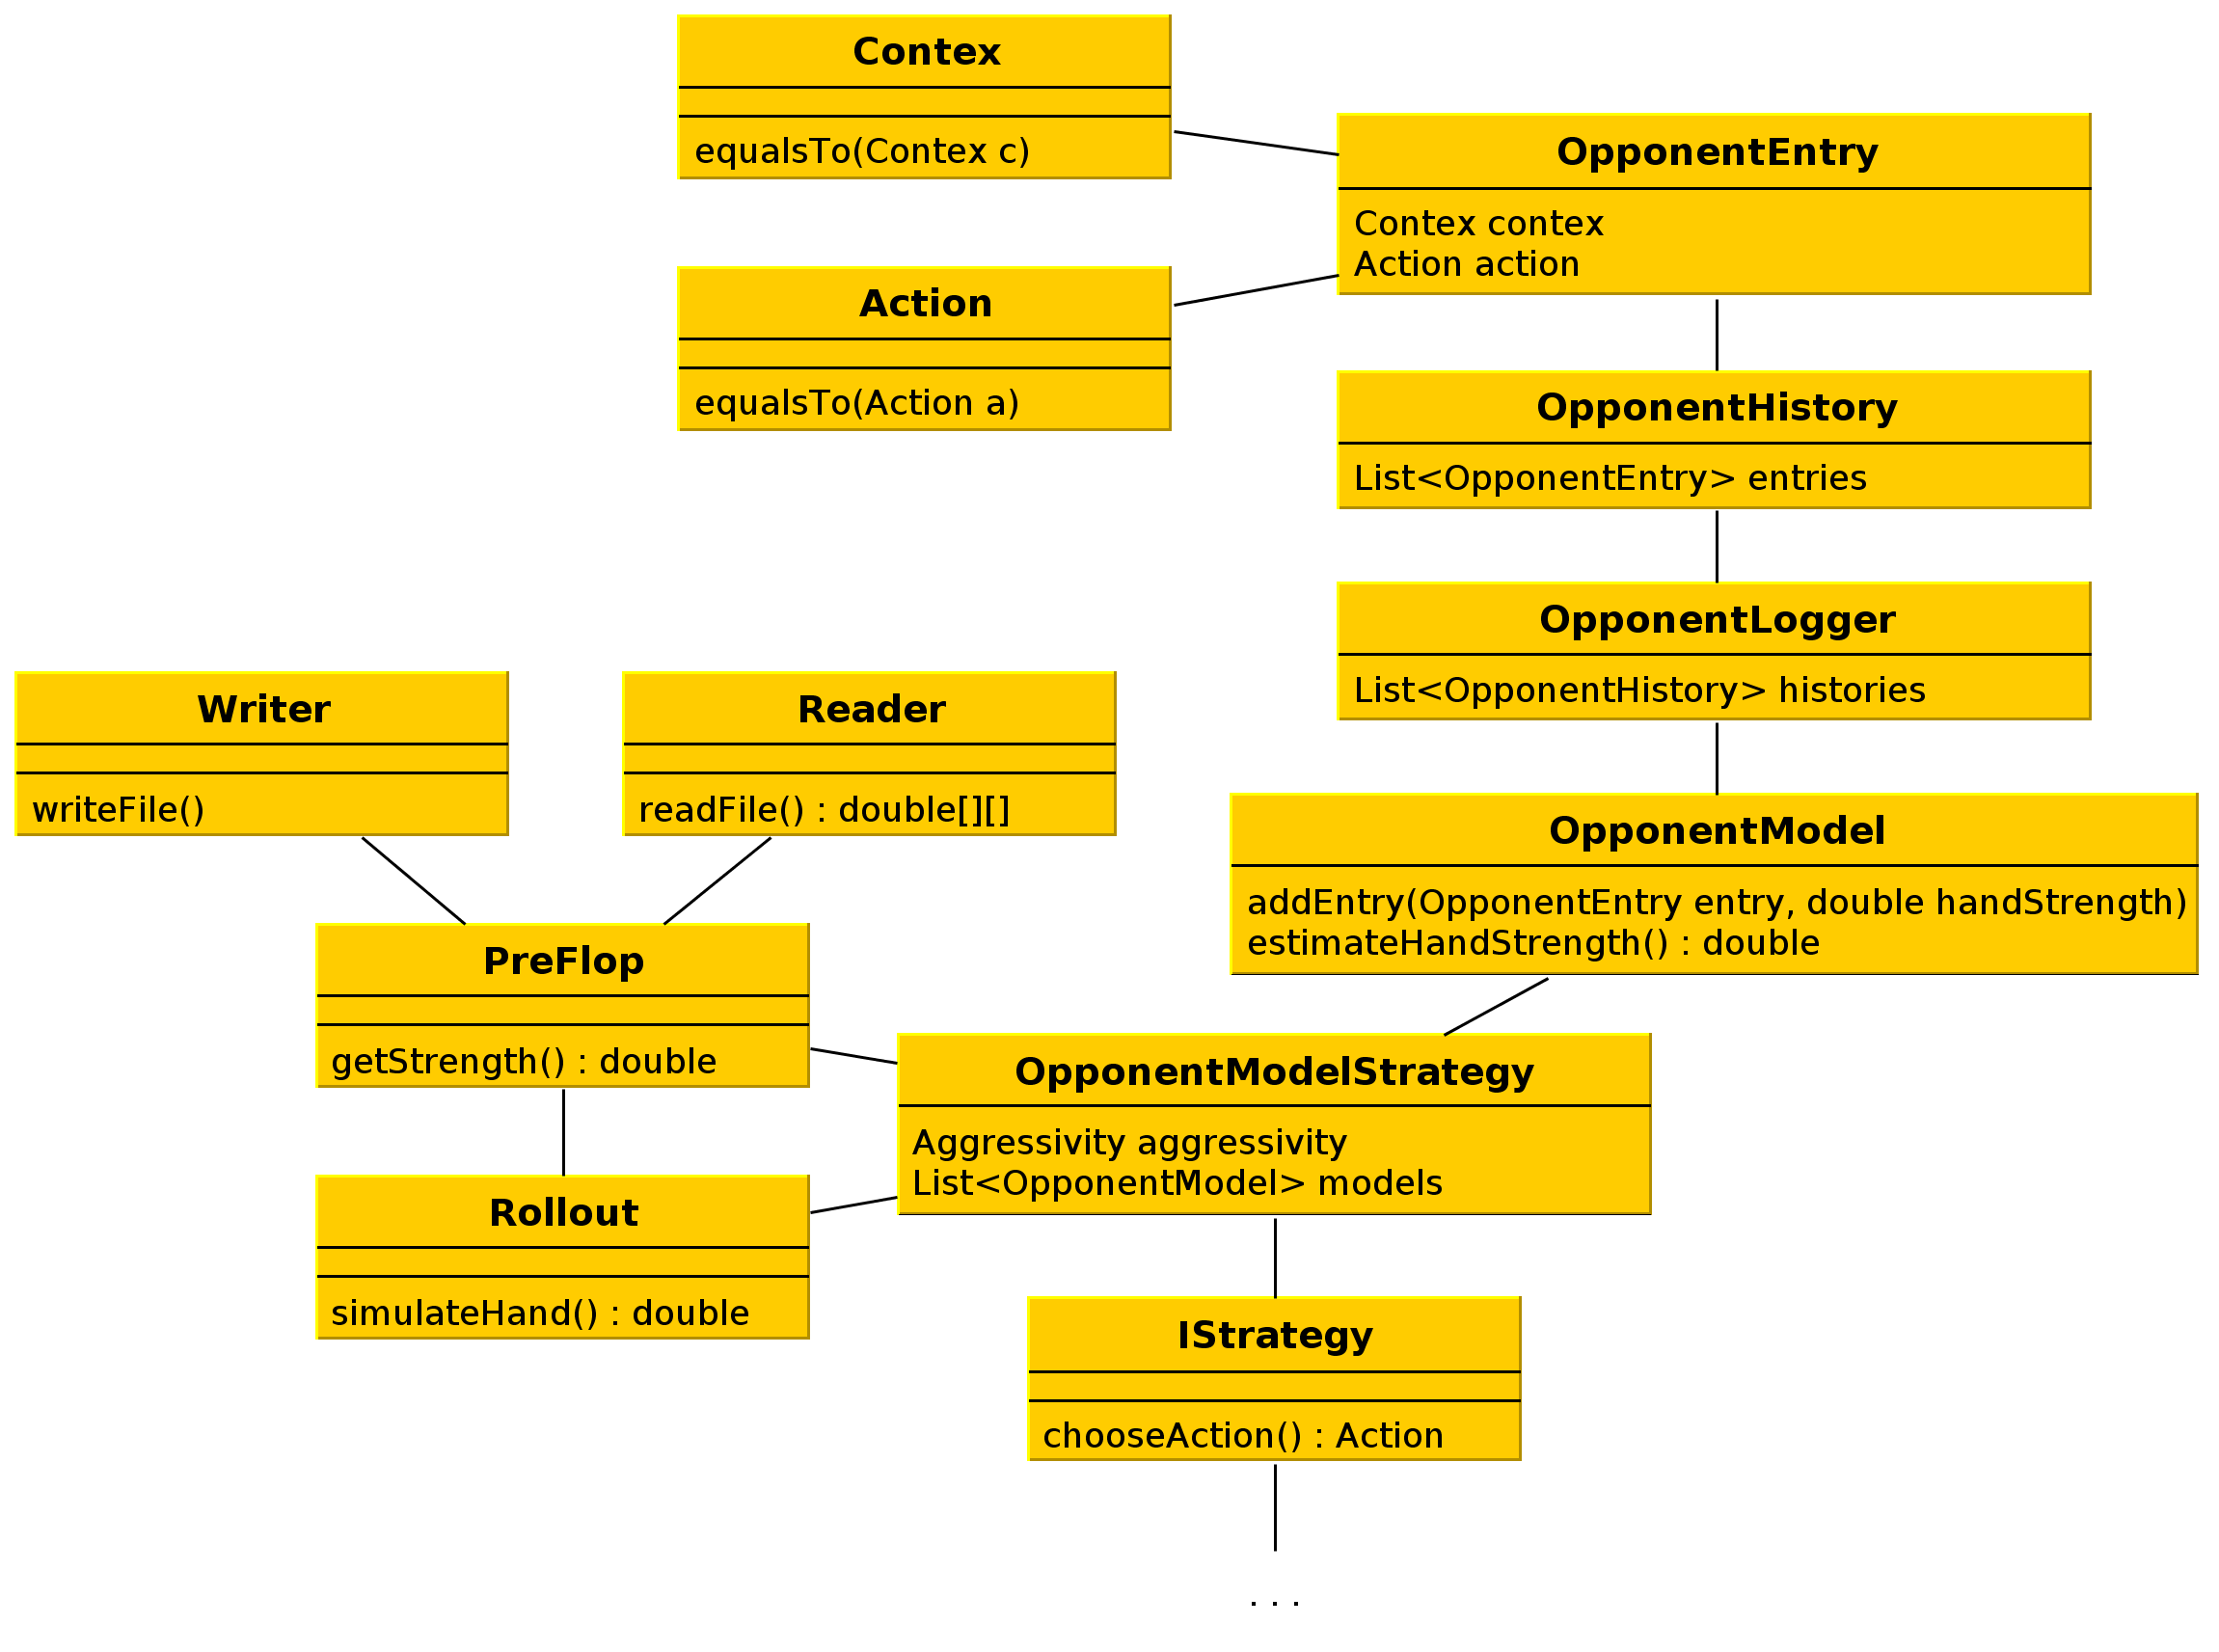
\includegraphics[width=1.0\textwidth]{images/phase3}
  \caption{Software design of phase III}
  \label{fig:phase3}
\end{figure}

\section{Model rules}
As mentioned above, the \emph{Opponent Model} contains  a triple of \emph{Context}, \emph{Player Action} and \emph{Hand Strength} of which the first two are again subdevided.

\subsection{Context}
The \emph{Context} can be considered as the state of the game at a specific point. Features that define a context are 
\begin{itemize}
	\item The stage, whether pre-flop, flop, turn or river
	\item The number of player that are still in the hand
	\item The number of raises during the current stage
	\item The pott odds
\end{itemize}

\subsection{Context}

\section{Opponent model strategy}
Basically the phase III player acts the same way like phase II player does. At first the amount that a player is willing to pay is calculated the same way. Afterwards the opponents' hand strengths are estimated. The player compares his own hand strengths with the estimated strengths and gets a number of players who are supposedly better and worse than him. These numbers are used to adjust the player's bet. The new bet is calculated as shown in \ref{equ:opponentModel1}, where $b'$ is the new bet, $b$ the old bet, $better$ the number of players who are better and $worse$ the number of player who are worse than the current player.

\begin{equation}
	\label{equ:opponentModel1}
	b' = b * (\frac{worse - better}{10})
\end{equation}

// TODO: contexts

\section{Results}

